\subsection{Problema a resolver}
El siguiente ejercicio consiste en hallar una manera de implementar un sistema proporcionado respetando una cota determinada de orden de complejidad. El problema se sitúa en un centro de distribución de correo que recibe paquetes todos los días cuyo destino final es la sede central de la empresa. Para el transporte de los mismos, éstos son cargados a camiones de igual capacidad. El encargado de logística, Pascual, tiene un sistema que utiliza desde hace años para agilizar la carga de los camiones asegurando el uso de una baja cantidad de los mismos para el envío de paquetes al final del día. Dicho sistema consiste en agarrar los paquetes y ubicarlos en algún camión que ya tenga paquetes dentro, eligiendo entre éstos el que menos peso esté cargando hasta ese momento. Si el peso del paquete permite que éste sea cargado en ese camión, se lo ubica allí, sino, se lo incluye en un nuevo camión.\newline
El problema a resolver se basa en escribir un algoritmo que tome los pesos de los paquetes que hay que acomodar e indique cuántos camiones se van a utilizar y cuánto peso se cargará en cada uno de ellos al final del día considerando el sistema de Pascual. Para esto, se respeta el orden de llegada de los paquetes a medida que ingresan. \newline
Las consideraciones a tener en cuenta son que los camiones tienen la misma capacidad de carga, la cantidad disponible de los mismos alcanza para transportar todos los paquetes y que el peso de un paquete no supera la capacidad de carga de un camión. Del mismo modo, el tamaño de los paquetes no es tenido en cuenta. Además, es importante tener en cuenta que las cargas son valores enteros positivos.\newline
\newline
\textbf {Formatos de entrada y salida:}\newline
\newline
La entrada contiene varias instancias del problema. Cada instancia consta de una línea con el siguiente formato:

$$L\ n\ p_{1}\ p_{2}\ ...\ p_{n}$$


donde \textbf{$L$} es el límite de carga de los camiones, \textbf{$n$} es la cantidad de paquetes a acomodar y \textbf{$p_{1}$, ..., $p_{n}$} son los pesos de cada paquete en el orden en el que deben ser almacenados.\newline

La salida debe contener una línea por cada instancia de entrada, con el siguiente formato:

$$k\ c_{1}\ c_{2}\ ...\ c_{n}$$


donde \textbf{$k$} es la cantidad de camiones utilizados y \textbf{$c_{1}$, ..., $c_{k}$} es el peso que se cargó en cada uno de los \textbf{$k$} camiones al final del día.\newline

En lo que sigue, presentaremos dos ejemplos sobre el sistema impulsado por Pascual:
\begin{itemize}
\item {\large{\textbf{Ejemplo 1:}}}\newline

En este ejemplo, decidimos conveniente develar un caso en el que fuera agregado un paquete a un camión ya cargado. Por otro lado, quisimos contrarrestarlo insertando un paquete con una carga que superaba la capacidad del camión creado anteriormente. Por último, nos pareció importante mostrar un caso en el que al agregar un nuevo paquete, si bien un nuevo camión había sido creado, éste era colocado en el camión cuya carga fuera la menor.\newline

\textbf{Formato de entrada:}
$$100\ \ 5\ \ 20\ \ 40\ \ 80\ \ 15\ \ 100$$

\begin{figure}[H] %[h] Aqui [b] para button [t] para top
\begin{center}
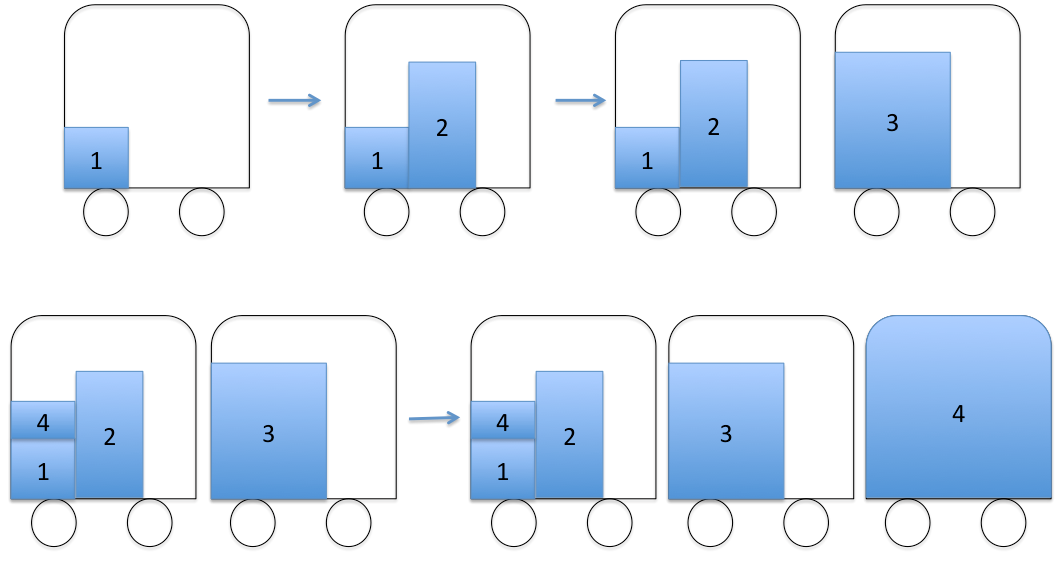
\includegraphics[width=320pt]{../imgs/ejemplo1.jpg}
\end{center}
\end{figure}

\textbf{Formato de salida:}
$$3\ \ 75\ \ 80\ \ 100$$


\item {\large{\textbf{Ejemplo 2:}}}\newline

En este ejemplo, quisimos mostrar lo que ocurría en caso en el que cada paquete superara el 50\% de la carga disponible en un camión.\newline

\textbf{Formato de entrada:} 
$$150\ \ 3\ \ 80\ \ 75\ \ 82$$

\begin{figure}[H] %[h] Aqui [b] para button [t] para top
\begin{center}
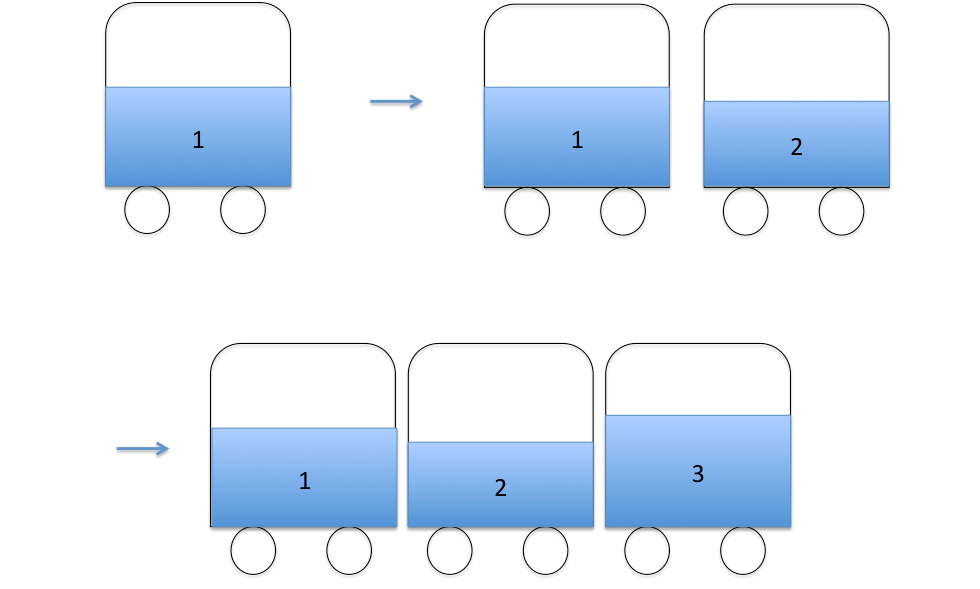
\includegraphics[width=300pt]{../imgs/ejemplo2.jpg}
\end{center}
\end{figure}

\textbf{Formato de salida:}
$$3\ \ 80\ \ 75\ \ 82$$


\end{itemize}
\subsection{Resolución coloquial}
Al analizar el problema a resolver, nos percatamos de que lo más conveniente era implementar la solución en base a un $algoritmo\ goloso$. Dicho algoritmo consiste en la construcción de una solución seleccionando, en cada paso, la mejor alternativa sin considerar las implicancias de ésta.\newline Por otro lado, dicha técnica de diseño algorítmico resulta fácil de implementar, suele ser eficiente y permite construir soluciones razonables.\newline
\newline
En este caso, la resolución basada en un algoritmo goloso nos permitió tomar cada instancia de la entrada y ubicarla en el lugar más conveniente en ese momento. Esto significa que dada la $i-ésima$ caja ingresada en un mismo día, ésta era ubicada en el camión que menor cargado se encontraba en el momento en el que se la agregaba. Para lograr esto, decidimos utilizar como estructura una cola de prioridad.\newline
\newline
Una cola de prioridad consiste en una estructura de datos en la que sus elementos son atendidos según la prioridad que éstos tengan asociada. Dicha estructura se caracteriza por admitir inserciones de nuevos elementos y la consulta y eliminación del elemento de mínima (o máxima) prioridad.\newline
Las colas de prioridad suelen ser útiles para resolver algoritmos golosos ya que éstos suelen tener una iteración principal, y una de las tareas a realizar en cada una de dichas iteraciones es seleccionar un elemento de entre varios que minimiza (o maximiza) un cierto criterio de optimalidad local.\newline
Para adaptar el problema de Pascual a la cola de prioridad, decidimos que cada elemento debía representar la capacidad de carga disponible correspondiente a un camión determinado en un momento dado junto con el orden de creación del mismo.\newline
\newline
El pseudocódigo ideado para resolver el problema es el siguiente:\newline

\begin{algorithm}[H]
	\SetAlgoLined
	\caption{Algoritmo de Pascual}
	\KwIn{Entero limite, Paquetes $ps$}
	\KwOut{cantidadDeCamiones, listaDePesos}
	\lIf{$ps = \emptyset$}{\textbf{devolver} 0, $ListaVacia$}\\
	
	Camiones $ca \leftarrow$ \{Camion $cNuevo(0)\}$\\
	cantidadDeCamiones := 1\\
	\For{Paquete p $\in$ $ps$}{
		Camion $c$ := camionMenosCargado\footnote{camionMenosCargado: Función que toma el camión menos cargado de la lista de camiones.}($ca$)\\
		\eIf{peso($p$)+capacidad($c$) $\leq$  limite}{
			capacidad($c$) $+=$ peso($p$)
		}{
			$ca \leftarrow$ Camion $cNuevo(0)$\\
			capacidad($cNuevo$) $=$ peso($p$)
			cantidadDeCamiones + 1;
		}
	}
	\textbf{devolver} cantidadDeCamiones, $ca$
\end{algorithm}

Como puede observarse en el pseudocódigo anterior, la función $cNuevo$ crea un nuevo camión cuya carga inicial es 0 (siendo ésta la misma para todos). Por otro lado, los paquetes que ingresan como parámetro se identifican por su peso.\newline
\newline
La función $camionMenosCargado$ devuelve el camión con mayor carga disponible. Dado que la estructura utilizada para almacenar los camiones provee dicha función, decidimos que no era necesario presentar el pseudocódigo de la misma.\newline


\subsection{Demostración de correctitud}

Para demostrar la correctitud de este problema definamos el invariante del algoritmo:
\begin{figure}[H] %[h] Aqui [b] para button [t] para top
\begin{center}
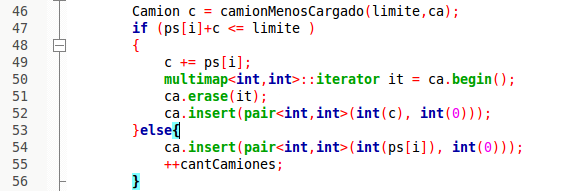
\includegraphics[width=300pt]{../imgs/demo11.jpg}
\end{center}
\end{figure}

\begin{itemize}
\item Cada camion leva hasta su limite en peso \\
Como se puede observar en la linea 47, la guarda no permite agregar un paquete tal que el mismo haga exceder el peso limite del camion.
\item Los paquetes se intentan agregar en los camiones ya llenos \\
 Se puede ver como en la linea 46 ya se toma el camion que este menos cargado (si es que existe), y si este puede contener el paquete, el mismo se agrega ahi. De no poder contenerlo lo pone en un camion nuevo. Lo que me asegura que no haya otro camion que pueda contener el paquete es, por un lado, el invariante de la estructura que estamos utilizando\footnote{http://en.cppreference.com/w/cpp/container/multimap}, y por otro, que si tomo el camion con mayor disponibilidad y no alcanza, los demas que tienen menos lugar, claramente tampoco van a poder llevar el paquete. 
\end{itemize}

Finalmente, sea $S$ una solucion del problema tal que contiene los camiones necesarios con sus cargas respectivas. Por nuestro invariante podemos asegurar que los camiones se van llenando segun el procedimiento explicitado por Pascual y por lo tanto la salida $S$ es correcta.


\subsection{Complejidad del algoritmo}
Tal como requerido, la complejidad temporal del algoritmo es estrictamente menor a $\mathcal{O}(n^2)$.


\subsection{Código fuente}



\subsection{Instancias posibles}



\subsection{Testing}
